\chapter{Extension of the Rule-Based Lloyd Algorithm to 3D\label{chap:rbl}}

\section{Introduction to the RBL}

    \subsection{Overview}
        The algorithm is a communication-less approach designed to navigate agents from point A to point B. 
        It relies on global positioning data, such as GPS or alternative methods for obtaining global coordinates, combined with sensor inputs that provide information about the agent's environment. 
        These sensors can include LiDAR, depth cameras, or standard cameras with estimation techniques, allowing the agent to detect and avoid obstacles or other agents. 
        The algorithm enables autonomous navigation without requiring direct communication between agents, making it suitable for scalable and decentralized applications.

    \subsection{Applications and Limitations in 2D}
        Modern robotics relies on the capability to navigate from point A to point B.
        Navigation plays a crucial role in various robotic applications, such as Automated Guided Vehicles (AGVs), which are commonly used in manufacturing and logistics. 
        AGVs typically follow predefined 2D trajectories guided by visual \cite{vision_navigation}, magnetic \cite{magnetic_navigation}, or LiDAR-based navigation \cite{lidar_navigation}. 
        Additionally, 2D navigation is widely employed in robotic vacuum cleaners, enabling them to systematically cover an area while avoiding obstacles.

        An obvious limitation for algorithms in 2D is scalability. 
        As the number of agents in a system increases, the complexity of managing their movements and coordination also grows significantly.
        Obstacle avoidance in 2D can also be less efficient compared to 3D environments, as agents have fewer options for evading obstacles. 
        In 3D, agents can change their altitude in addition to their horizontal trajectory, giving them more freedom to maneuver around obstacles.

    \subsection{Key principles}
        RBL, as presented in the original paper \cite{rbl_paper}, ensures convergence to the goal and provides sufficient conditions for achieving it. 
        The problem involves individual control of $N$ agents from their initial position $\mathbf{p}_i(0)$ toward a goal region, represented as circle.
        This goal region is denoted as $B(\mathbf{e}_i, \epsilon)$, where $\mathbf{e}_i$ is center and $\epsilon$ is radius of goal region.
        Each agent is knows of its current position $\mathbf{p}_i$, encumbrance $\delta_i$, which determines safe space around agent.
        Additionally, each agent also knows the positions and encumbrances of its neighboring agents $\mathbf{\mathcal{N}_i}$, agent $j \in \mathbf{\mathcal{N}_i}$ if $||\mathbf{p}_i - \mathbf{p}_j|| \leq 2r_{s,i}$, where $r_{s,i}$ is denoted as half of the sensing radius of the i-th agent.
        For simplicity $r_{s,i}$ is considered to be same for all agents, therefore $r_{s,i} = r_s$. 

        The core objective of the algorithm is to minimize the coverage cost function, which accounts for the distribution of agents and obstacles over the environment. 
        This function is expressed as:
        \begin{equation}
            J_{cov}(\mathbf{p}) = \sum_{i=1}^{N} \int_{\mathcal{V}_i} \lVert\mathbf{q}-\mathbf{p}_i\rVert^2 \phi_i (\mathbf{q})d\mathbf{q},
            \label{coverage_cost_function}
        \end{equation}
        where $\mathbf{p}_i$ is the position of agent $i$, $\mathcal{V}_i$ is the Voronoi cell of the i-th robot, $\lVert\mathbf{q}-\mathbf{p_i}\rVert^2$ is squared Euclidian distance between point in the mission space $\mathbf{q} \in \mathcal{Q}$ and agent's position $p_i$, 
        and $\phi_i (\mathbf{q})$ is the weighting function.

        Voronoi cell is defined as: 
        \begin{equation}
            \mathcal{V}_i = \{q \in \mathcal{Q} \lvert \lVert \mathbf{q} - \mathbf{p}_i \rVert \leq \lVert q - \mathbf{p}_j \rVert, \forall j \neq i\}
        \end{equation}
        For visual representation see \reffig{fig:voronoi_2d}. 
        However, this standard definition of Voronoi cells does not take into account the physical space occupied by the agents, or their encumbrances. 
        To address this, a Modified Voronoi cell is introduced, which takes into account the encumbrances of agents.
        This modified version adjusts the boundaries of each Voronoi cell to account for the encumbrances of neighboring agents.
        The modified Voronoi cell definition is as follows:
        \begin{equation}
            \tilde{V}_i = 
            \begin{cases}
            \{ \mathbf{q} \in Q \mid \| \mathbf{q} - \mathbf{p}_i \| \leq \| \mathbf{q} - \mathbf{p}_j \| \}, & \text{if } \Delta_{ij} \leq \frac{\| \mathbf{p}_i - \mathbf{p}_j \|}{2} \\
            \{ \mathbf{q} \in Q \mid \| \mathbf{q} - \mathbf{p}_i \| \leq \| \mathbf{q} - \tilde{\mathbf{p}}_j \| \}, & \text{otherwise},
            \end{cases}
        \end{equation}
        $\forall j \in \mathcal{N}_i$, where $\Delta_{ij} = \delta_i + \delta_j$ and $\tilde{\mathbf{p}}_j = \mathbf{p}_j + 2(\Delta_{ij} - \frac{\| \mathbf{p}_i - \mathbf{p}_j \|}{2})\frac{ \mathbf{p}_i - \mathbf{p}_j }{\| \mathbf{p}_i - \mathbf{p}_j \|}$.
        Together with cell $\mathcal{S}_i$ defined as: 
        \begin{equation}
            \mathcal{S}_i = \{\mathbf{q} \in \mathcal{Q} | \| \mathbf{q} - \mathbf{p}_i \| \leq r_{s,i}\}
        \end{equation}
        we get cell $\mathcal{A}_i = \tilde{V}_i \cap \mathcal{S}_i$ .
        \begin{figure}[H]
            \centering
            \subfloat[Euclidean Voronoi Diagram in 2D] {
            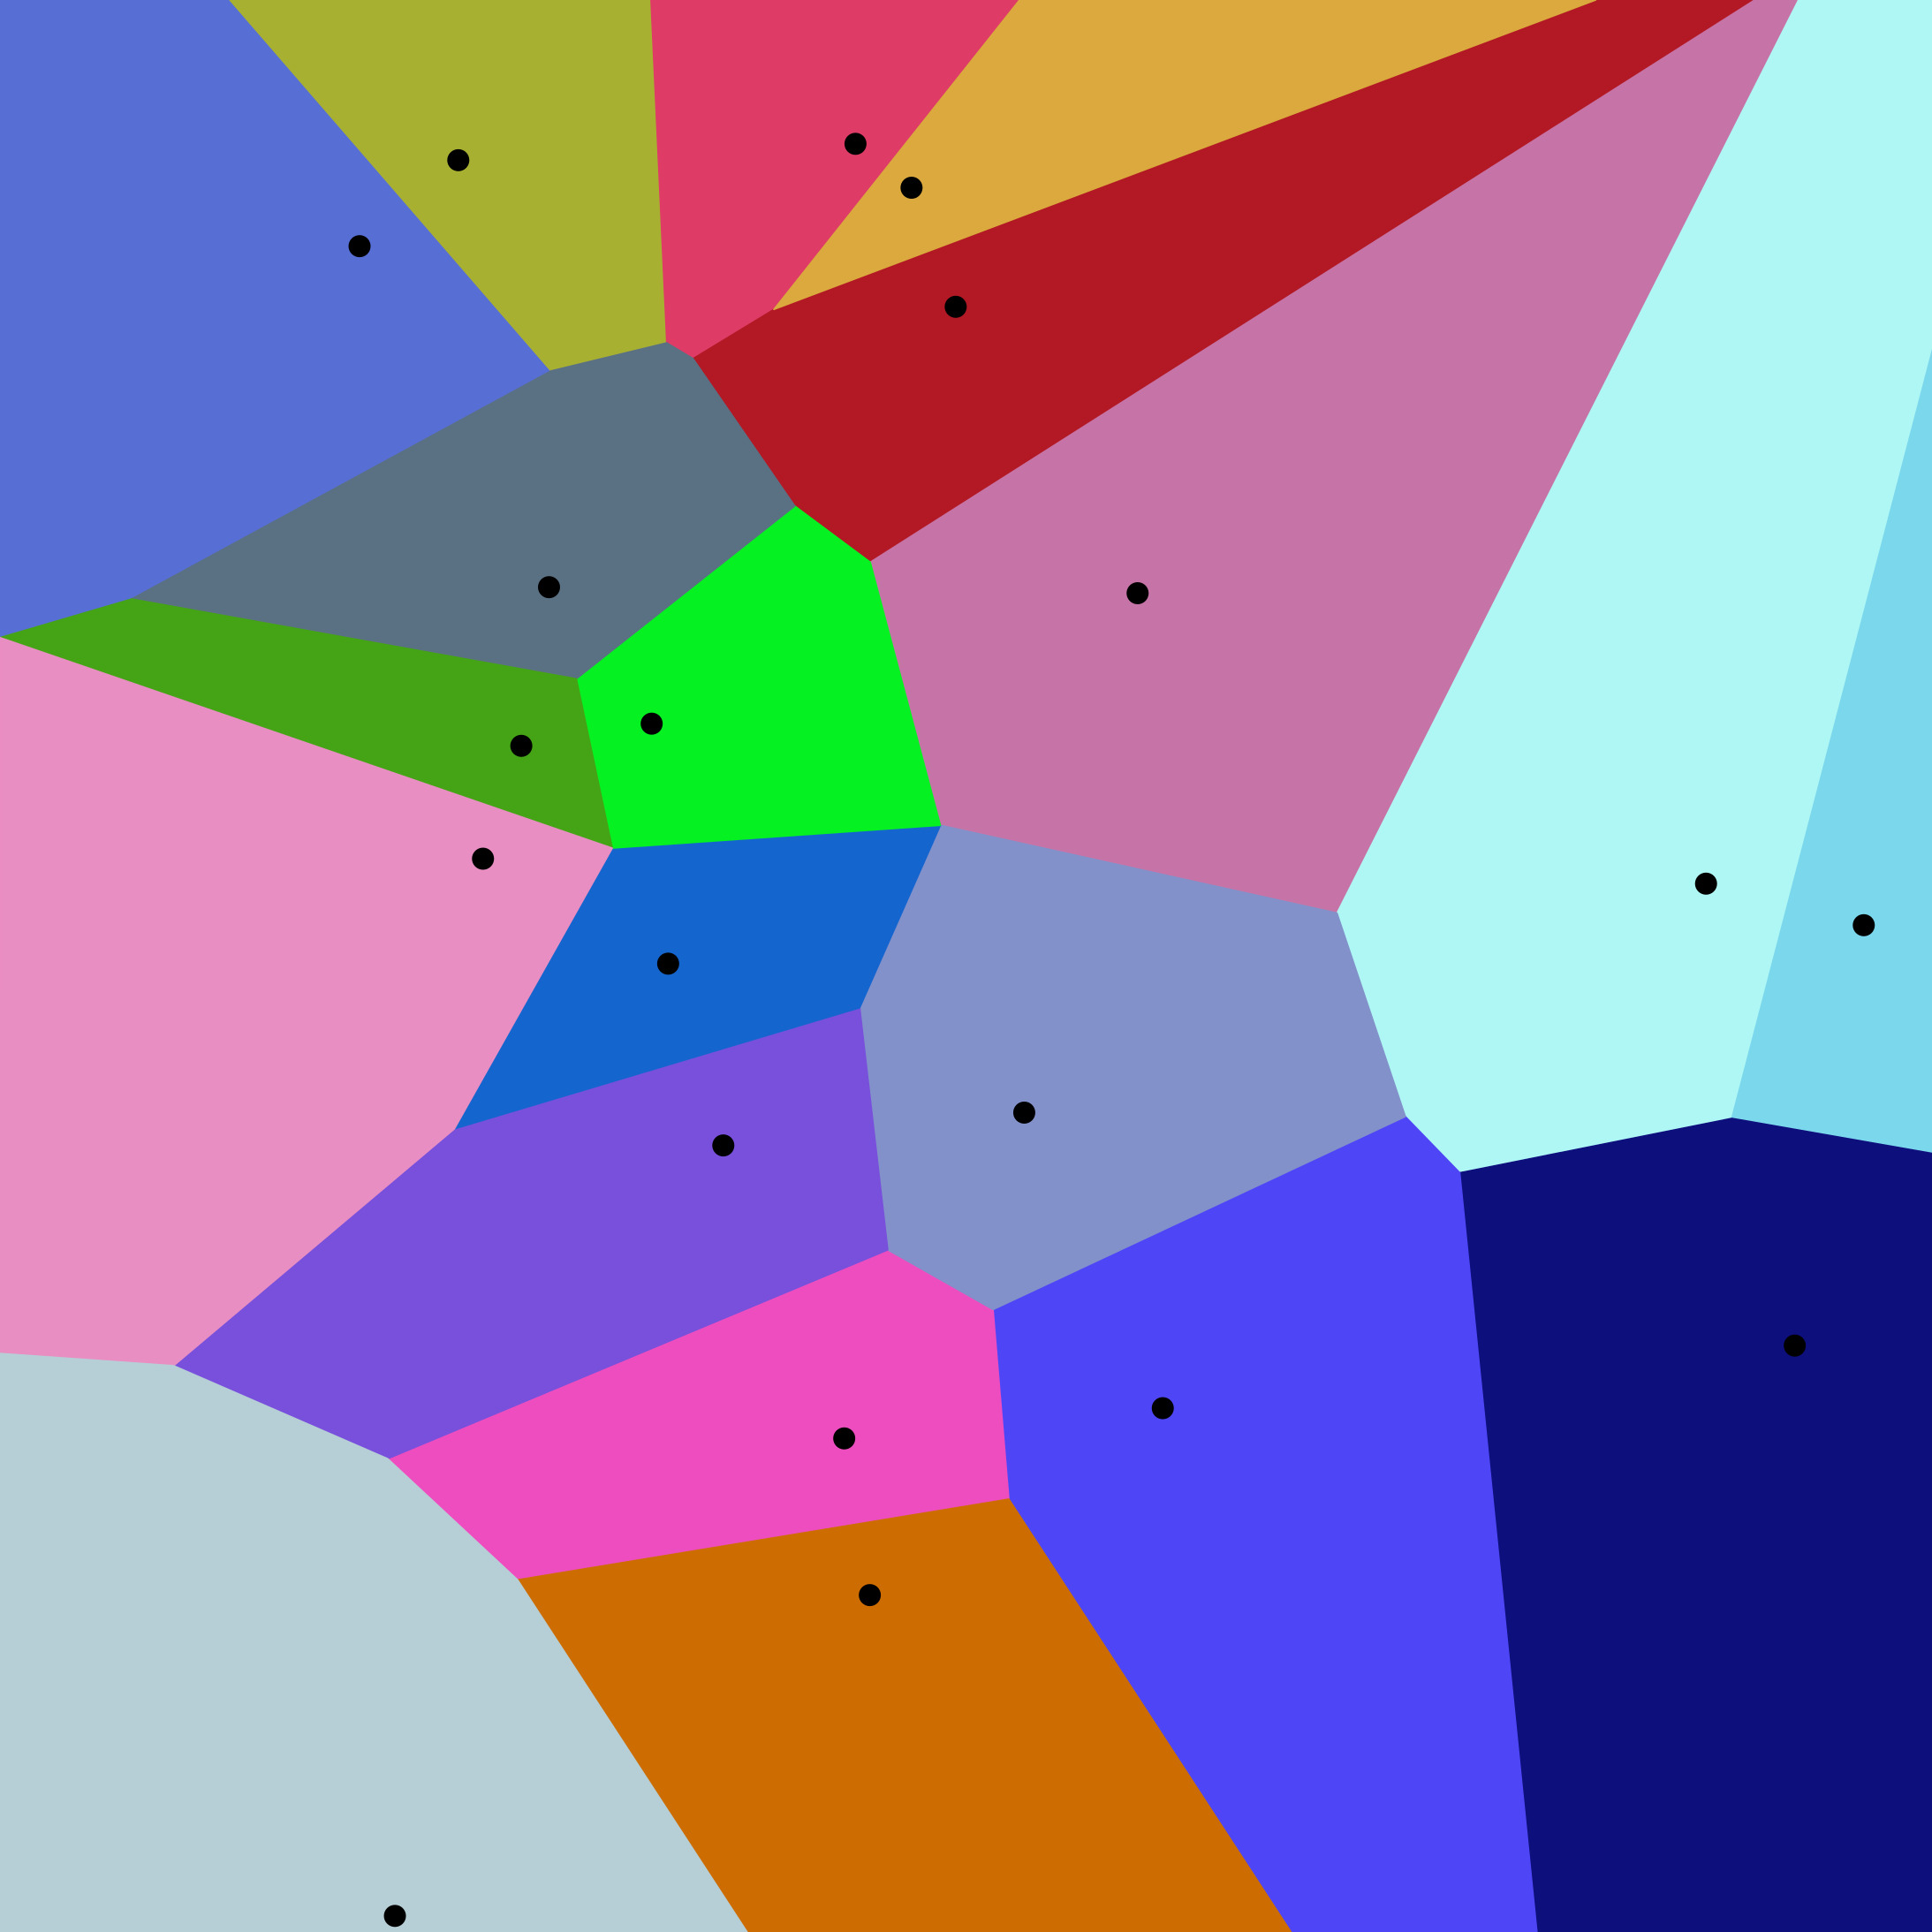
\includegraphics[width=0.48\textwidth, height=0.48\textwidth]{./fig/diagrams/Euclidean_Voronoi_diagram.jpg}
            \label{fig:voronoi_2d}
            }
            \subfloat[Euclidean Voronoi Diagram in 3D] {
            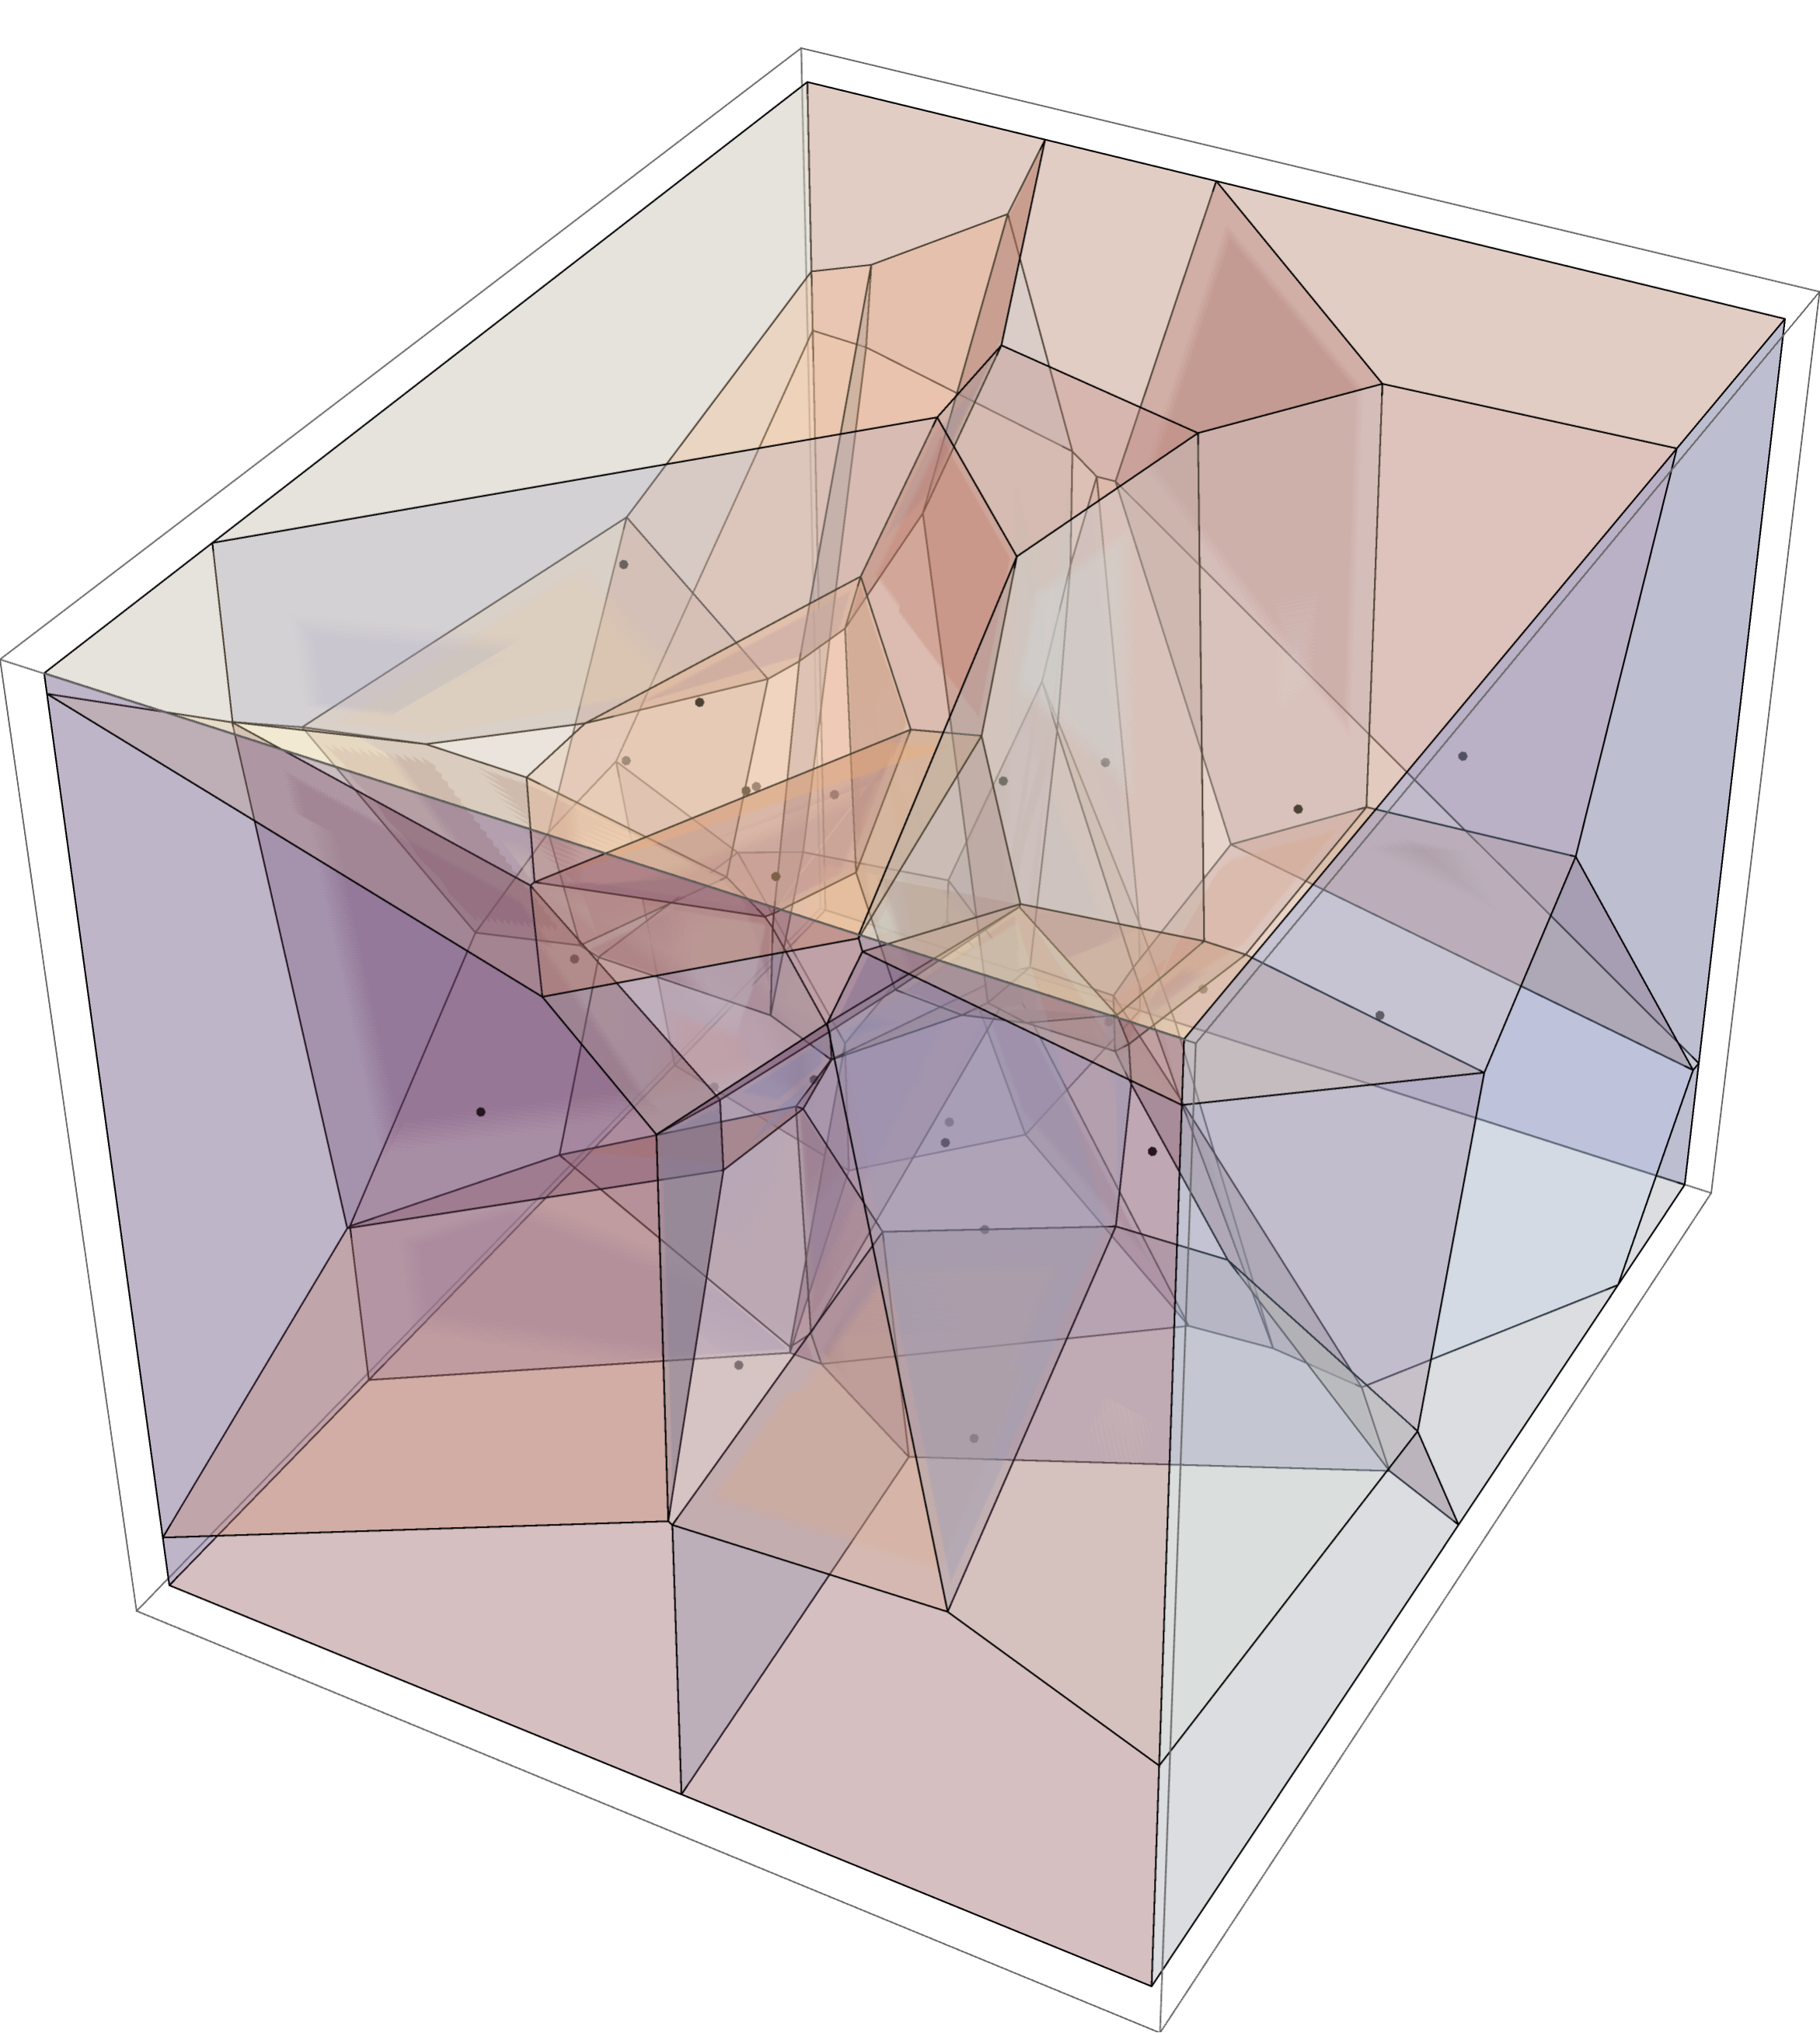
\includegraphics[width=0.48\textwidth, height=0.48\textwidth]{./fig/diagrams/Euclidian Voronoi diagram 3d.png}
            \label{fig:voronoi_3d}
            }
            \caption{
                (a) an example of 20 Voronoi cells in 2D \cite{Voronoi2d} (b) 25 Voronoi cells in 3D \cite{Voronoi3d}
            }
            \label{fig:voronoi_diagrams}
        \end{figure}

        Convergence to goal region $B(\mathbf{e}_i, \epsilon)$ depends on the choice of weighting function that assigns weights to points $\mathbf{q}$ in the mission space $\mathcal{Q}$.
        The weighting function $\phi_i(\mathbf{q})$ is defined as follows: 
        \begin{equation}
            \phi_i(\mathbf{q}) = \exp\left(-\frac{\|\mathbf{q} - \mathbf{\bar{p}}_i\|}{\beta_i}\right),
        \end{equation}
        where 
        
        \begin{equation}
            \dot{\beta}_i(A_i) = 
            \begin{cases}
                -\beta_i & \text{if } \|\mathbf{c}_{A_i} - \mathbf{p}_i\| < d_1 \land \|\mathbf{c}_{A_i} - \mathbf{c}_{S_i}\| > d_2, \\
                -(\beta_i - \beta_i^D) & \text{otherwise.}
            \end{cases}
        \end{equation}
        
        \begin{equation}
            \mathbf{\dot{\bar{p}}}_i = 
            \begin{cases}
                -(\mathbf{\bar{p}}_i - R^{\mathbf{p}_i} (\frac{\pi}{2} - \epsilon) \mathbf{e}_i) & \text{if } \|\mathbf{c}_{A_i} - \mathbf{p}_i\| < d_3 \land \|\mathbf{c}_{A_i} - \mathbf{c}_{S_i}\| > d_4, \\
                -(\mathbf{\bar{p}}_i - \mathbf{e}_i) & \text{otherwise,}
            \end{cases}
        \end{equation}
        
        \[
            \mathbf{\bar{p}}_i = 
            \begin{cases}
            \mathbf{e}_i & \text{if } \|\mathbf{p}_i - \mathbf{c}_{\mathcal{A}_i}\| > \|\mathbf{p}_i - \mathbf{c}_{\mathcal{A}_i}\|, \\
            R^{\mathbf{p}_i} (\frac{\pi}{2} - \epsilon) \mathbf{e}_i & \text{otherwise.}
            \end{cases}
        \]
            

        
        The position of the centroid \( \mathbf{c}_{V_i} \) of a region \( V_i \), weighted by the function \( \phi_i(\mathbf{q}) \), is used to guide the control. It is defined as:

        \begin{equation}
            \mathbf{c}_{V_i} = \frac{\int_{V_i} \mathbf{q} \phi_i(\mathbf{q}) \, d\mathbf{q}}{\int_{V_i} \phi_i(\mathbf{q}) \, d\mathbf{q}},
        \end{equation}

        where \( \mathbf{q} \) represents the position vector, and \( \phi_i(\mathbf{q}) \) is a weighting function. 
        The centroid \( \mathbf{c}_{V_i} \) serves as the target for the control system, directing the system toward the weighted center of the region.

    \section{Motivation for 3D Extension}
        In many practical applications, agents must operate in three-dimensional spaces, considering not only horizontal movement but also vertical positioning.
        A 3D extension is necessary to navigate complex environments that feature obstacles in all directions.
        In 2D, agents are restricted to a flat plane, which simplifies navigation but limits the ability to interact with objects and environments that exist in the third dimension.
        The ability to utilize vertical space can enhance energy efficiency, as agents can optimize their paths by ascending or descending to avoid obstacles or to find more favorable environmental conditions, such as discovering more open space.

    \section{Mathematical Describtion in 3D}

    modified voronoi partitioning, transition from planar 2d to spatial 3d, safety and convergence in 3d.

    \section{Simulation and Results Analysis}

    Describtion of simulation enviroment, used tools, Describtion of few simulation scenarios and result analysis.

    \section{Summary and Key Insights}

    Recap of modifications. Faced challenges and solutions applied
